\section{Stellar Mass Completeness} \label{sec:mscomp}
In this appendix, we describe how we derive $M_{\rm lim}$, the $M_*$ limit
above which our BGS Bright sample is complete. 
Although there are various methods for estimating $M_{\rm lim}$ in the
literature, \emph{e.g.} based on estimating the mass-to-light
ratio~\citep{pozzetti2010, moustakas2013}, we adopt a simple approach that
takes advantage of the fact that BGS Bright is a magnitude-limited sample. 

\begin{figure}
\begin{center}
    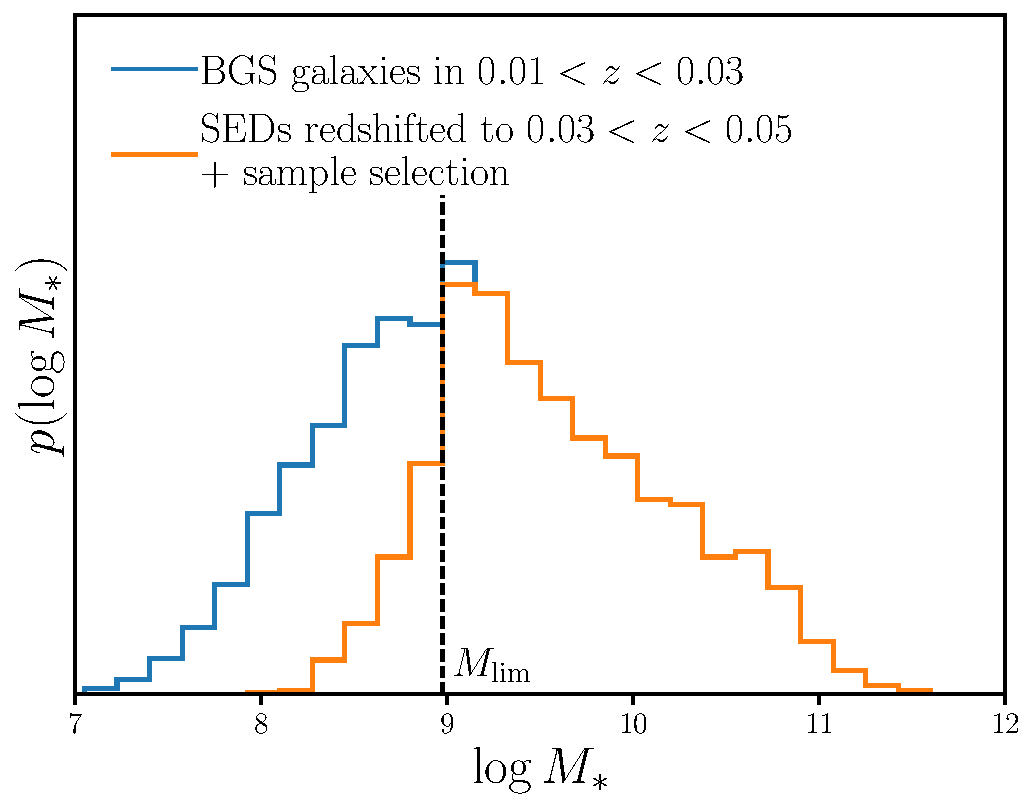
\includegraphics[width=0.45\textwidth]{figs/psmf_logMstar_comp_demo.pdf}
    \caption{
        The $M_*$ distribution of BGS Bright galaxies with $0.01 < z < 0.03$
        (blue) and the $M_*$ distribution of same set of galaxies that would
        remain in the BGS Bright magnitude limit if they were redshifted to 
        $z' = z + 0.02$: $r' < 19.5$. 
        We set the stellar mass completeness limit, $M_{\rm lim}$, for $0.01 <
        z < 0.05$ to the $M_*$ where more than 10\% of galaxies are excluded in
        the latter distribution. 
    }\label{fig:ms_comp0}
\end{center}
\end{figure}

To derive $M_{\rm lim}$ in redshift bins of width $\Delta z=0.04$, we first
split the galaxy sample into narrower bins of $\Delta z/2$. 
For each narrower redshift bin, $i \Delta z/2 < z < (i+1) \Delta z/2$, we take
all the best-fit {\sc PROVABGS} SEDs from all  galaxies in the bin and
artificially redshift it to $z' = z + \Delta z/2$:
\begin{equation}
    f_\lambda' = f_\lambda \frac{d_L(z)^2}{d_L(z')^2}.
\end{equation} 
$d_L(z)$ reprents the luminosity distance at redshift $z$. 
Afterward, we calculate the $r$-band magnitudes, $r'$, for $f_\lambda'$ and
impose the $r' < 19.5$ magnitude limit of the BGS Bright. 
We then compare the $M_*$ distribution of all the galaxies in 
$i \Delta z/2 < z < (i+1) \Delta z/2$ to the galaxies in 
$i \Delta z/2 < z < (i+1) \Delta z/2$ with $r' < 19.5$.
For instance,  we present the $M_*$ distributions of all BGS
Bright galaxies in $0.01 < z < 0.03$ (blue) and the BGS Bright galaxies in
$0.01 < z < 0.03$ with $r' < 19.5$ (orange) in Figure~\ref{fig:ms_comp0}.

\begin{table} 
    \caption{Stellar mass completeness limit, $M_{\rm lim}$ for redshift bins
    of width $\Delta z = 0.04$.} 
    \begin{center}
        \begin{tabular}{lc} \toprule
            $z$ range & $\log_{10} M_{\rm lim}$ \\[3pt]
            \hline 
            $0.01 - 0.05$   & 8.975 \\ 
            $0.05 - 0.09$   & 9.500 \\ 
            $0.09 - 0.13$   & 10.20 \\ 
            $0.13 - 0.17$   & 10.38 \\ 
            $0.17 - 0.21$   & 10.72 \\ 
            \hline            
\end{tabular} \label{tab:mscomp}
\end{center}
\end{table}

\begin{figure}[h]
\begin{center}
    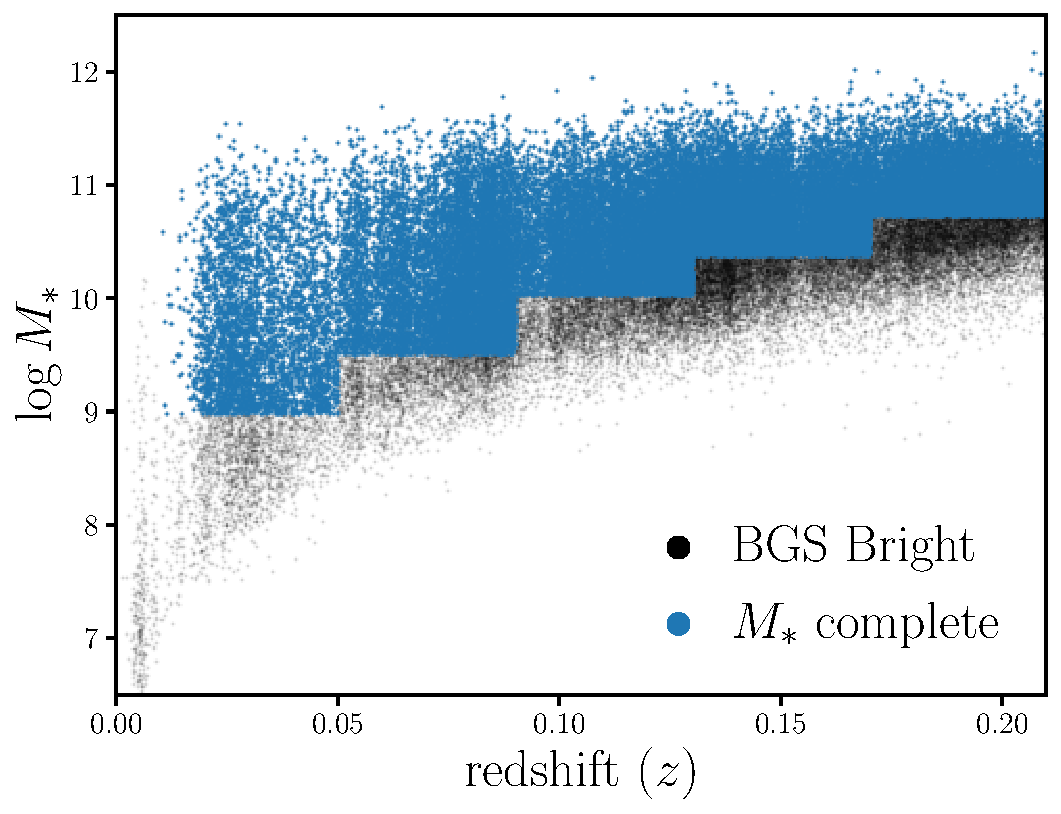
\includegraphics[width=0.6\textwidth]{figs/psmf_logMstar_comp_z.pdf}
    \caption{
        $M_*$ and redshift relation of BGS Bright galaxies in the EDR (black)
        and the galaxies within the stellar mass completeness limit ($M_* <
        M_{\rm lim}$; blue). 
        $M_{\rm lim}$ is derived in redshift bins of width $\Delta z = 0.04$. 
        The lowest redshift bin ($0.01 < z < 0.05$) is complete down to 
        $M_* < 10^9 M_\odot$. 
    }\label{fig:ms_comp1}
\end{center}
\end{figure}

Since galaxies become fainter when they are placed at higher redshifts,
\emph{i.e.} $r' > r$, the $r' < 19.5$ sample has fewer low $M_*$ galaxies. 
We determine the $M_*$ at which, more than 10\% of galaxies are excluded in the
$r' < 19.5$ sample (black dashed) and set this limit as $M_{\rm lim}$ for the
redshift bins: $0.01 < z < 0.05$.
Our procedure for deriving $M_{\rm lim}$ takes advantage of the fact that
galaxy samples at lower redshifts are complete down to lower $M_*$ than at
higher redshifts. 
We repeat this procedure for all the $\Delta z = 0.04$ redshift bins that we
use to measure the SMF.
In Table~\ref{tab:mscomp}, we list $M_{\rm lim}$ values for each of the
redshift bins. 
Furthermore, we present the $M_*$ and redshift relation of BGS Bright galaxies
(black) and the stellar mass complete sample (blue) in
Figure~\ref{fig:ms_comp1}. 
